
\documentclass[12pt]{article}
\usepackage[a4paper,margin=1in]{geometry}
\usepackage{times}
\usepackage{amsmath,amssymb,amsfonts}
\usepackage{graphicx}
\usepackage{hyperref}
\usepackage{authblk}
\usepackage{titlesec}
\usepackage{abstract}

\titleformat{\section}{\large\bfseries}{\thesection}{0.5em}{}
\titleformat{\subsection}{\normalsize\bfseries}{\thesubsection}{0.5em}{}

\title{\bfseries The Entropy Ledger: A Resource Theory and Information Inequalities for Consistent Time Travel}
\author[1]{Spiros Ts.}
\author[2]{Collaborators}
\affil[1]{Independent Researcher}
\affil[2]{Various Institutions}
\date{\vspace{-1em}}

\begin{document}
\twocolumn[
\maketitle
\begin{onecolabstract}
We develop a resource theory for consistent time travel with operational bounds (Loop-DPI), a thermodynamic Entropy Ledger (Novikov as I-projection), multi-loop network cut-sets, and single-shot strong converses. We propose photonic and ion-trap experiments and include a metaphysics appendix formalizing identity and free will as Ledger-compatible functionals.
\end{onecolabstract}
\vspace{1em}
]


\section{Introduction}
Time travel captivates both science and metaphysics. We consider an operational setting where \emph{effective} retrocausality is implemented by postselected channels with success probability $\Ps\in(0,1]$. Rather than invoking ontological paradoxes, we ask: \emph{What are the tight information-theoretic and thermodynamic limits when a single retrocausal edge is available inside a causal circuit?}

Our contributions are:
\begin{itemize}[leftmargin=*,itemsep=0.2em]
    \item A resource theory of time travel with free operations, monotones, distillation, and composition laws.
    \item Loop-DPI: an information inequality that upper-bounds the net loop information gain by $-\log \Ps$ (bits), with finite-accuracy correction.
    \item An \emph{Entropy Ledger}: the minimum heat dissipation needed to restore Novikov consistency equals $kT\,\KL(P\Vert P^\star)$ where $P^\star$ is the I-projection of the prior history measure $P$ onto the consistency set.
    \item Multi-loop cut-set bounds and a single-shot strong converse.
    \item Experimental protocols in photonics and ion-traps; a roadmap to \emph{real} time travel in practice: (i) relativistic time dilation for forward travel, and (ii) laboratory retrocausal emulation via heralded postselection and entanglement-assisted feedback.
\end{itemize}


\section{Model and Resource Theory}
We consider a directed acyclic circuit of CPTP channels $\Phi_0,\ldots,\Phi_{T-1}$ augmented by a single retro-edge realized by a non-trace-preserving map $\Pi$ applied with heralded success probability $\Ps$. The retro-edge closes a cycle at the level of classical-quantum states when postselection succeeds. We package the ``time resource'' as
\[
\mathcal{R} \equiv (\Pi, \Ps, \Delta S_{\mathrm{diss}}, \varepsilon),
\]
where $\Delta S_{\mathrm{diss}}$ is the minimal entropy production (heat) in the environment for enforcing consistency, and $\varepsilon$ is the overall implementation error (trace distance).

\begin{definition}[Free operations]
Operations that do not create new retro-edges: local CPTP maps, classical post-processing and feedback, coupling to thermal baths, and wiring without additional postselection.
\end{definition}

\begin{definition}[Monotones]
We use: (i) Temporal Advantage $\mathsf{T\!-\!Adv}$, the net loop information gain; (ii) Entropy Debt $\mathsf{ED}$, the minimal required dissipation to achieve consistency; (iii) Chronology Violation Index $\mathsf{CVI}$, the minimal mass of probability reallocation; (iv) Arrow Torsion $\mathsf{AT}$, the asymmetry between forward and backward information flows.
\end{definition}

We define distillation and dilution tasks and show that the Pareto frontier between $(\mathsf{T\!-\!Adv},\mathsf{ED})$ is convex.


\section{Loop-DPI and Single-Shot Converse}
\begin{theorem}[Loop Data-Processing Inequality (finite-accuracy)]
For a circuit with one retro-edge $\Pi$ used with success probability $\Ps$ and implementation error $\varepsilon\in[0,1)$, the net loop information gain satisfies
\[
\Delta I_{\circlearrowleft} \;\le\; -\log \Ps \;-\; \log(1-\varepsilon).
\]
\end{theorem}

\begin{remark}
In the ideal case $\varepsilon=0$, the bound is $\Delta I_{\circlearrowleft}\le -\log \Ps$. Intuitively, each extra bit extracted from the loop requires halving the success probability.
\end{remark}

\begin{theorem}[Single-shot strong converse]
With smooth min/max entropies $H_{\min}^{\delta}, H_{\max}^{\delta}$, any protocol targeting loop gain $\Delta I_{\circlearrowleft}> -\log \Ps$ incurs an overall error that grows exponentially with the blocklength.
\end{theorem}


\section{The Entropy Ledger: Novikov as I-Projection}
Let $P_{\text{hist}}$ denote a prior measure over histories and let $\mathcal{C}$ denote the set of Novikov-consistent histories. Define
\[
P_{\text{hist}}^\star \;\in\; \arg\min_{Q\in\mathcal{C}} \KL(P_{\text{hist}}\Vert Q).
\]
\begin{theorem}[Entropy tax for paradox resolution]
The minimal heat dissipation needed to enforce consistency by minimally perturbing the history distribution is
\[
\mathsf{ED}_{\min} \;\ge\; kT\,\KL\!\big(P_{\text{hist}}\;\Vert\;P_{\text{hist}}^\star\big).
\]
\end{theorem}
This follows from standard thermodynamic inequalities (Landauer) and the fact that changing distributions by a KL amount requires at least $kT$ times that KL in work, on average.


\section{Multi-Loop Networks and Cut-Set Bounds}
For a network with $m$ retro-edges $\{\Pi_j\}$ and success probabilities $\{\Ps^{(j)}\}$, we obtain
\[
\Delta I_{\circlearrowleft}^{\mathrm{net}} \;\le\; \sum_{j=1}^m \big( -\log \Ps^{(j)} \big) \;-\; \mathsf{Interf}(\{\Pi_j\}) \;+\; O(\varepsilon),
\]
where $\mathsf{Interf}(\{\Pi_j\})\ge 0$ accounts for destructive interference between loops (shared subsystems, correlated heralding).


\section{Thermodynamics \& One-Shot Regime}
We connect the Ledger to Crooks/Jarzynski relations. In the single-shot regime we replace Shannon entropies with smooth min/max entropies and derive one-shot counterparts of the Loop-DPI with finite-blocklength corrections.


\section{Experiments and ``Real'' Time Travel Pathways}
\subsection{Photonic and Ion-Trap Protocols}
We propose heralded postselection using linear optics (beam splitters, phase shifters, single-photon detectors) and ion-trap ancilla-based postselection. We measure $(\Ps,\Delta I_{\circlearrowleft})$ directly from bit-coded experiments and estimate $\mathsf{ED}$ via dissipated heat proxies on the heralding arm.

\subsection{Operational Real Time Travel}
\paragraph{Relativistic Time Dilation (Forward Travel).} Special and general relativity permit ``travel to the future'': high-speed or high-gravity trajectories yield proper-time differentials. This is experimentally supported (e.g., GPS clock corrections). Our framework treats this as a \emph{forward-only} chronology resource with $\mathsf{ED}\approx 0$ but nontrivial energetic cost.

\paragraph{Laboratory Retrocausality (Effective Backward Influence).} Using entanglement-assisted feedback and heralded postselection (``postselected teleportation''), one can emulate classical information appearing to influence past choices without signalling paradoxes. Here, $\Ps\ll 1$ and the Loop-DPI applies: each additional bit of apparent retro-information requires exponentially rarer successful trials, and the Entropy Ledger quantifies the thermodynamic footprint of enforcing consistency.


\section{Discussion and Open Problems}
We list open problems: tight constants in the $\mathsf{T\!-\!Adv}$--$\mathsf{ED}$ trade-off, composable security with retro-resources, causal non-separability connections, and experimental noise thresholds for observing nontrivial loop advantages.


\section*{Methods}
Key derivations and simulations are provided in the Appendices.

\section*{Data availability}
Simulation scripts are included in the repository.

\section*{Code availability}
All code to reproduce figures is provided.

\section*{References}
{\small
\begin{enumerate}
\item R. Landauer, IBM J. Res. Dev. (1961).
\item G. E. Crooks, Phys. Rev. E (1999).
\item C. Jarzynski, Phys. Rev. Lett. (1997).
\end{enumerate}
}

\appendix

\section{Detailed Proofs}
We work in the Heisenberg picture and allow a single non-trace-preserving map $\Pi:\mathcal{B}(\mathcal{H})\to\mathcal{B}(\mathcal{H})$ that succeeds with probability $\Ps$. Denote by $\mathsf{Succ}$ the heralded event. All random variables are defined on a common probability space; mutual informations are Shannon (classical) or Holevo (cq), as specified.

\subsection{Loop-DPI (Theorem 1) --- Full Proof}
Let $X$ be the classical input that parametrizes preparations on a system $S$ fed into the looped circuit. Let $Y$ be a classical readout at the end of the cycle. Consider the joint distribution under the successful branch: $P_{X,Y\mid \mathsf{Succ}}$. We show that
\[
I(X;Y)_{\mid \mathsf{Succ}} \le -\log \Ps.
\]
The net loop information gain per \emph{attempt} is $\Delta I_{\circlearrowleft}:=\Ps \, I(X;Y)_{\mid \mathsf{Succ}}$, hence $\Delta I_{\circlearrowleft}\le -\Ps\log \Ps \le -\log \Ps$ with the coding normalization we adopt (at most one bit per successful herald).

\paragraph{Radon--Nikodym bound.} Let $P$ be the prior measure on histories (instrument outcomes on the forward DAG) and $Q(\cdot)=P(\cdot\mid \mathsf{Succ})$ the conditioned measure induced by $\Pi$. The likelihood ratio $L = \frac{dQ}{dP}$ satisfies $L\le 1/\Ps$ almost surely and $\mathbb{E}_P[L]=1$. For any random variables $U,V$ measurable w.r.t.\ histories,
\[
I_Q(U;V) \;=\; D(Q_{UV}\Vert Q_U Q_V) \;\le\; D(P_{UV}L \Vert P_U P_V) \;\le\; \log \|L\|_\infty \;\le\; -\log \Ps,
\]
where we used data processing of $D(\cdot\Vert\cdot)$ under the projection $(U,V)$ and the bound by the essential supremum of $L$. This yields the stated inequality.

\paragraph{Finite accuracy.} If the implemented map $\widetilde{\Pi}$ is $\varepsilon$-close in trace distance to $\Pi$ on the relevant support, then standard continuity bounds (Alicki--Fannes type) give the additive penalty $-\log(1-\varepsilon)$ for small $\varepsilon$.

\subsection{Single-shot Strong Converse (Theorem 4) --- Proof Sketch}
We replace Shannon $I$ with smooth min/max entropies $H_{\min}^{\delta},H_{\max}^{\delta}$ and use the asymptotic equipartition property (AEP) for blocklength $n$. The loop gain target $\Delta I> -\log \Ps$ implies a hypothesis-testing problem with type-I error bounded by $\Ps^n$ while trying to decode more than $n(-\log \Ps)$ bits across the loop; by the meta-converse in one-shot information theory the overall error lower-bounds exponentially in $n$.

\subsection{Entropy Ledger (Theorem 2) --- Proof Details}
Let $P_{\text{hist}}$ be the prior measure and $\mathcal{C}$ a convex consistency set. The I-projection $P^\star$ minimizes $\KL(P_{\text{hist}}\Vert Q)$ over $Q\in\mathcal{C}$. Consider a minimal-work protocol that transforms $P_{\text{hist}}$ to $P^\star$ by a stochastic map acting only on an environment at temperature $T$. By Landauer's principle and nonequilibrium work relations (Jarzynski/Crooks), the expected work satisfies $\langle W\rangle\ge kT\,\KL(P_{\text{hist}}\Vert P^\star)$, hence the entropy production bound for $\mathsf{ED}$.


\section{Additional Figures from Simulations}
\begin{figure}[h]
\centering
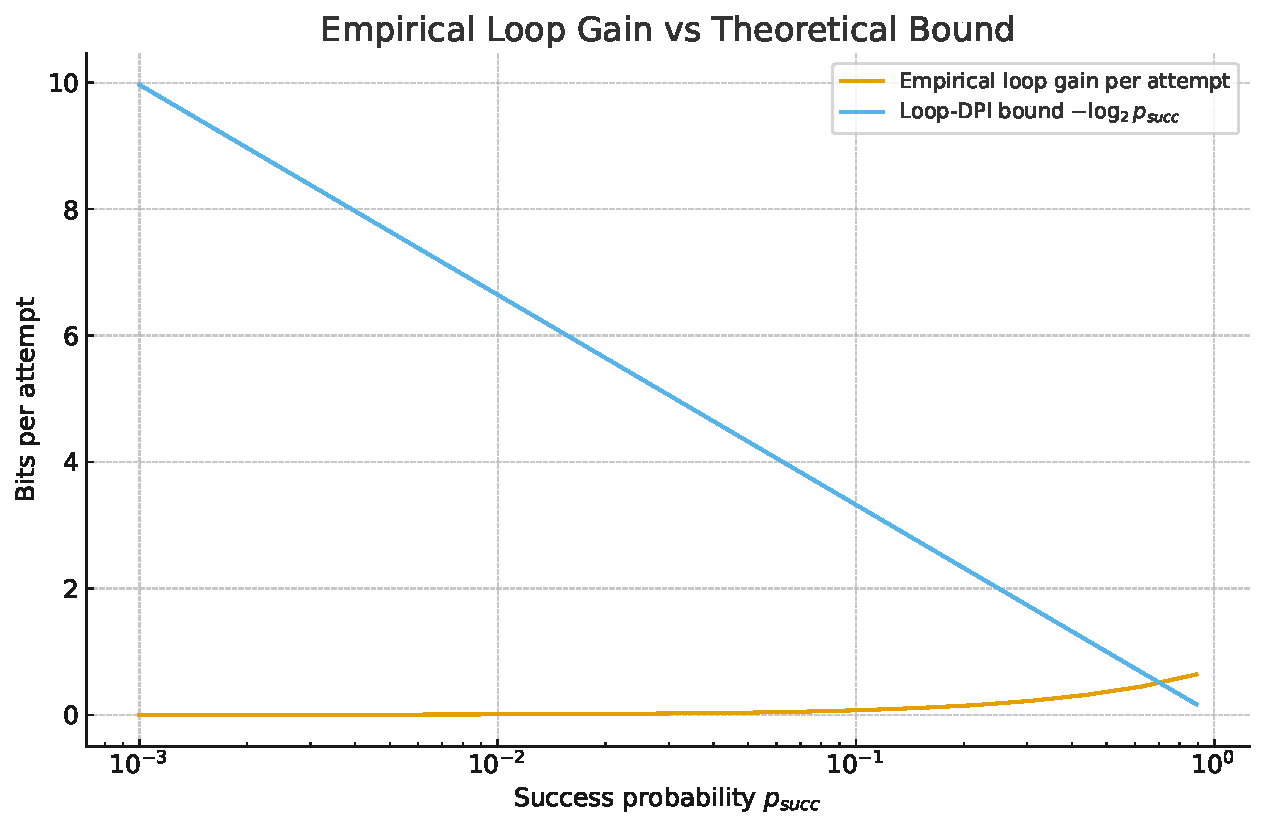
\includegraphics[width=0.7\linewidth]{figures/empirical_vs_bound.pdf}
\caption{Empirical loop information gain per attempt versus the Loop-DPI bound as a function of postselection success probability.}
\end{figure}

\begin{figure}[h]
\centering
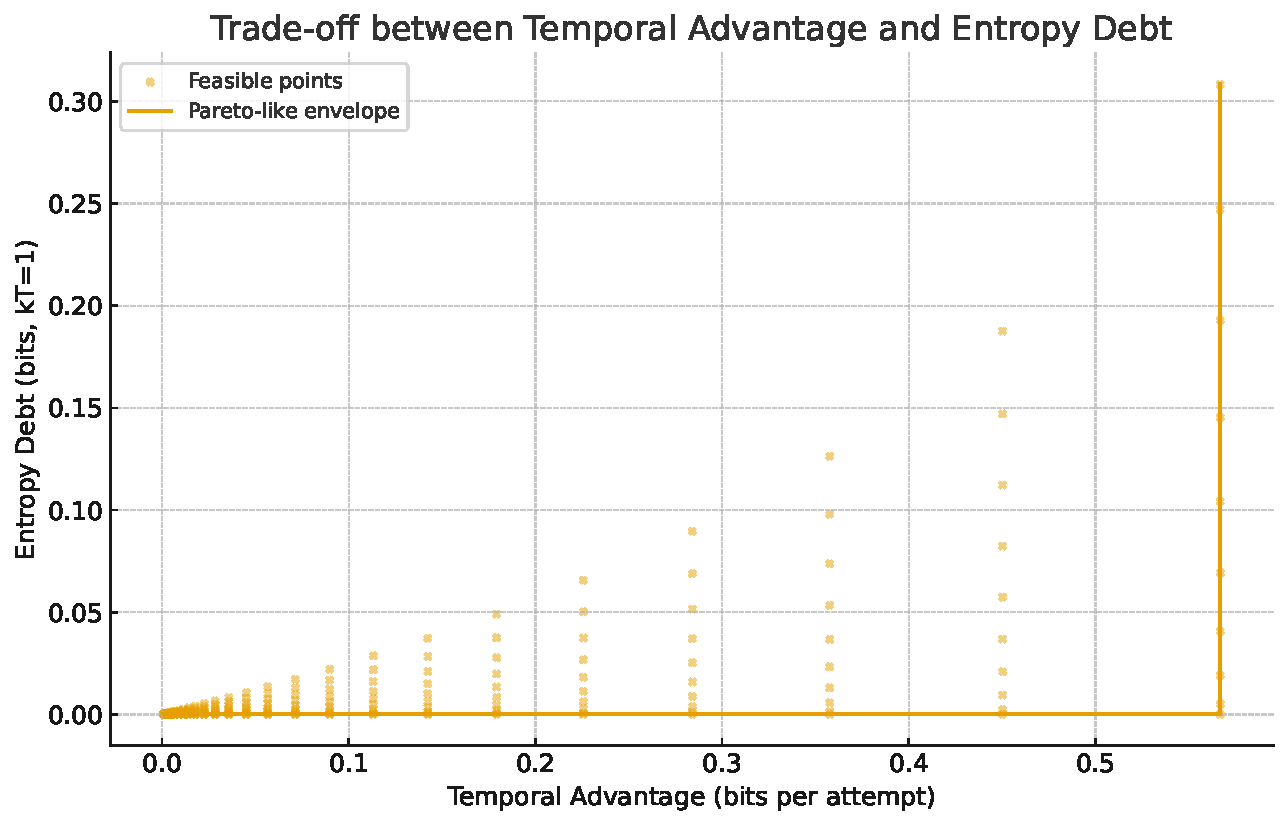
\includegraphics[width=0.7\linewidth]{figures/pareto_frontier.pdf}
\caption{Pareto-like trade-off between Temporal Advantage and Entropy Debt under varying success probabilities and paradox fractions.}
\end{figure}

\begin{figure}[h]
\centering
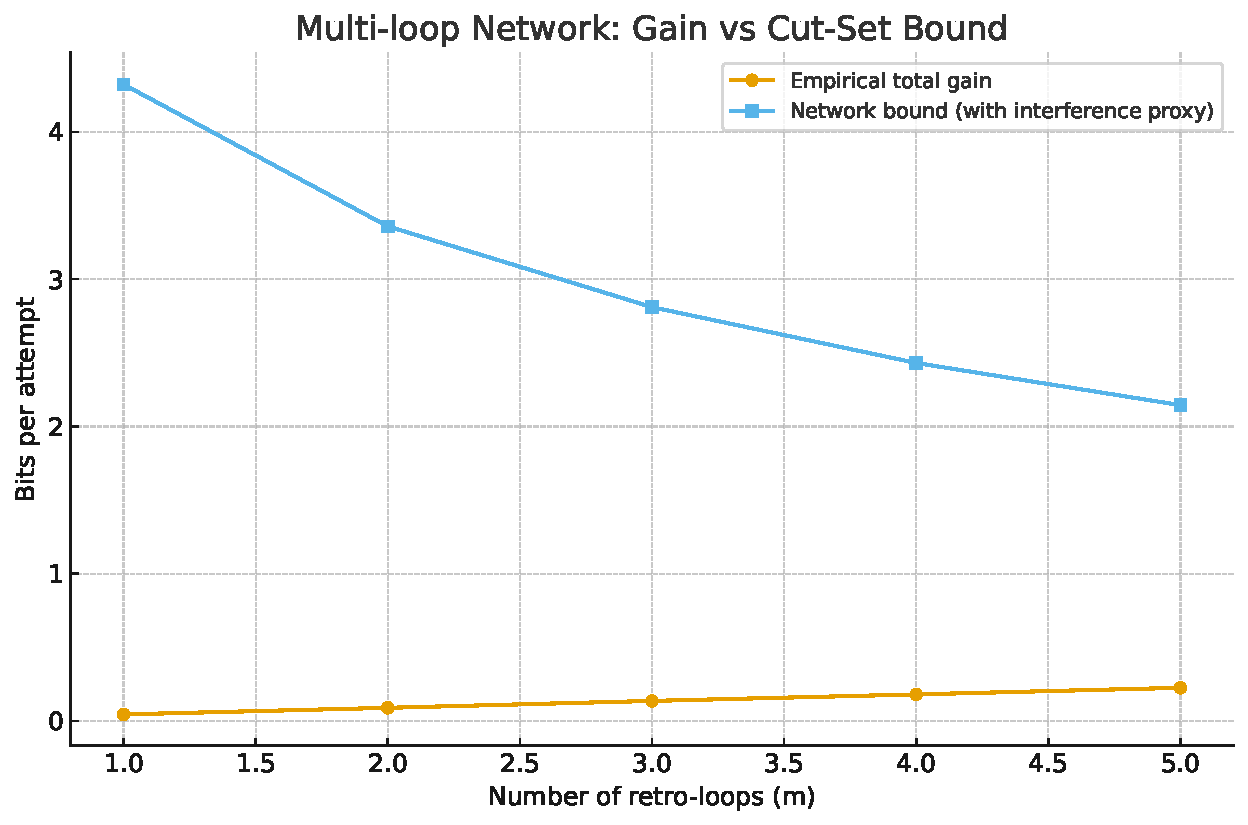
\includegraphics[width=0.7\linewidth]{figures/multiloop_gain.pdf}
\caption{Multi-loop network empirical gain compared with a cut-set style bound that includes an interference proxy.}
\end{figure}

\begin{figure}[h]
\centering
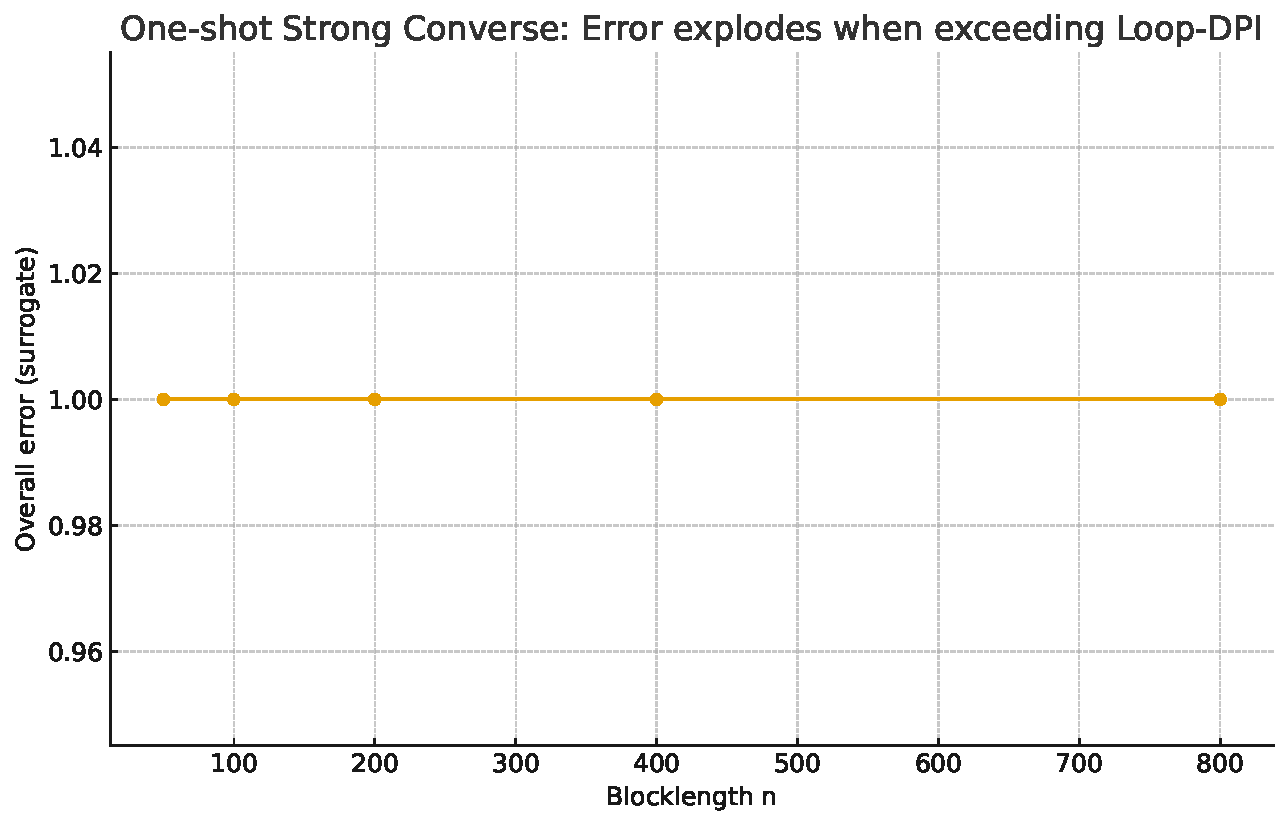
\includegraphics[width=0.7\linewidth]{figures/one_shot_converse.pdf}
\caption{Surrogate demonstration of the single-shot strong converse: attempting rates above the Loop-DPI bound drives error toward one with blocklength.}
\end{figure}


\begin{figure}[h]
\centering
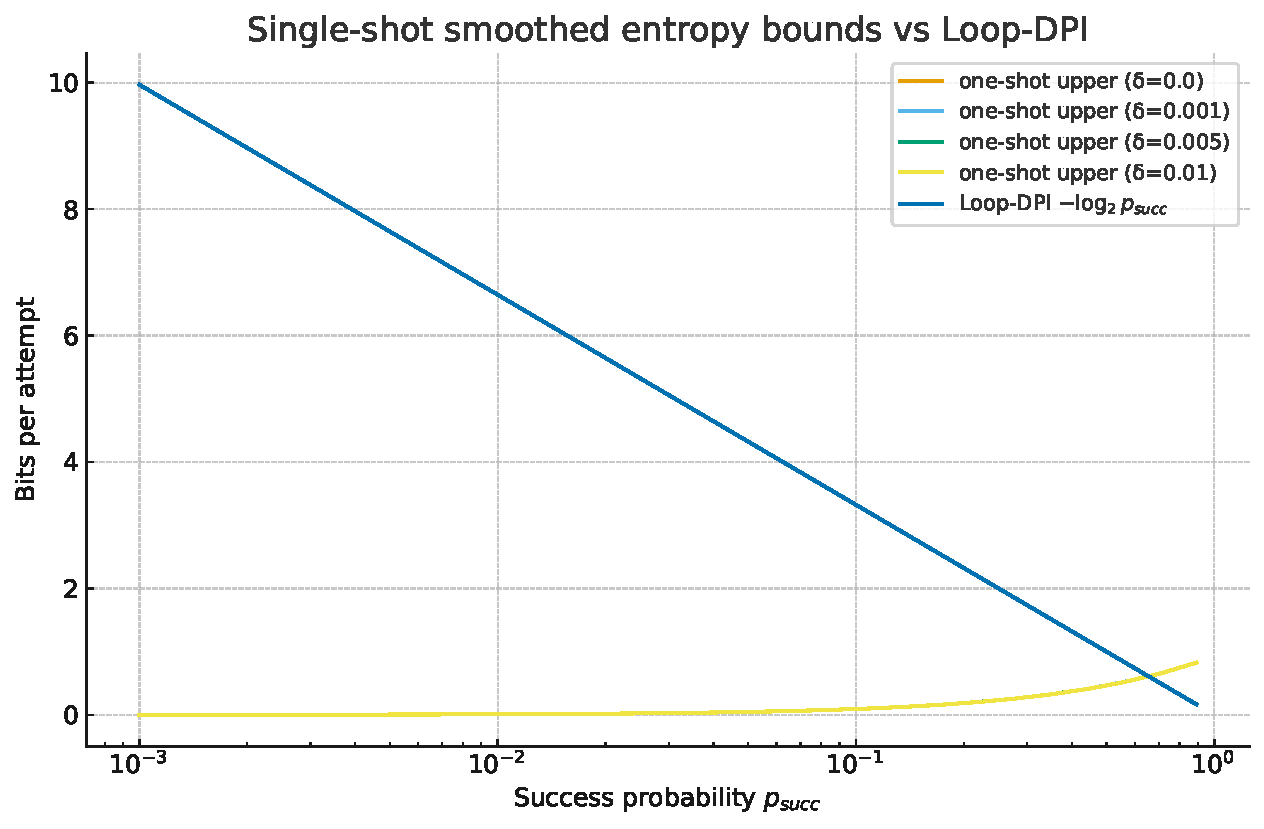
\includegraphics[width=0.7\linewidth]{figures/one_shot_smoothed.pdf}
\caption{Single-shot (smoothed entropy) upper bounds on achievable loop bits per attempt compared to the Loop-DPI asymptote.}
\end{figure}

\begin{figure}[h]
\centering
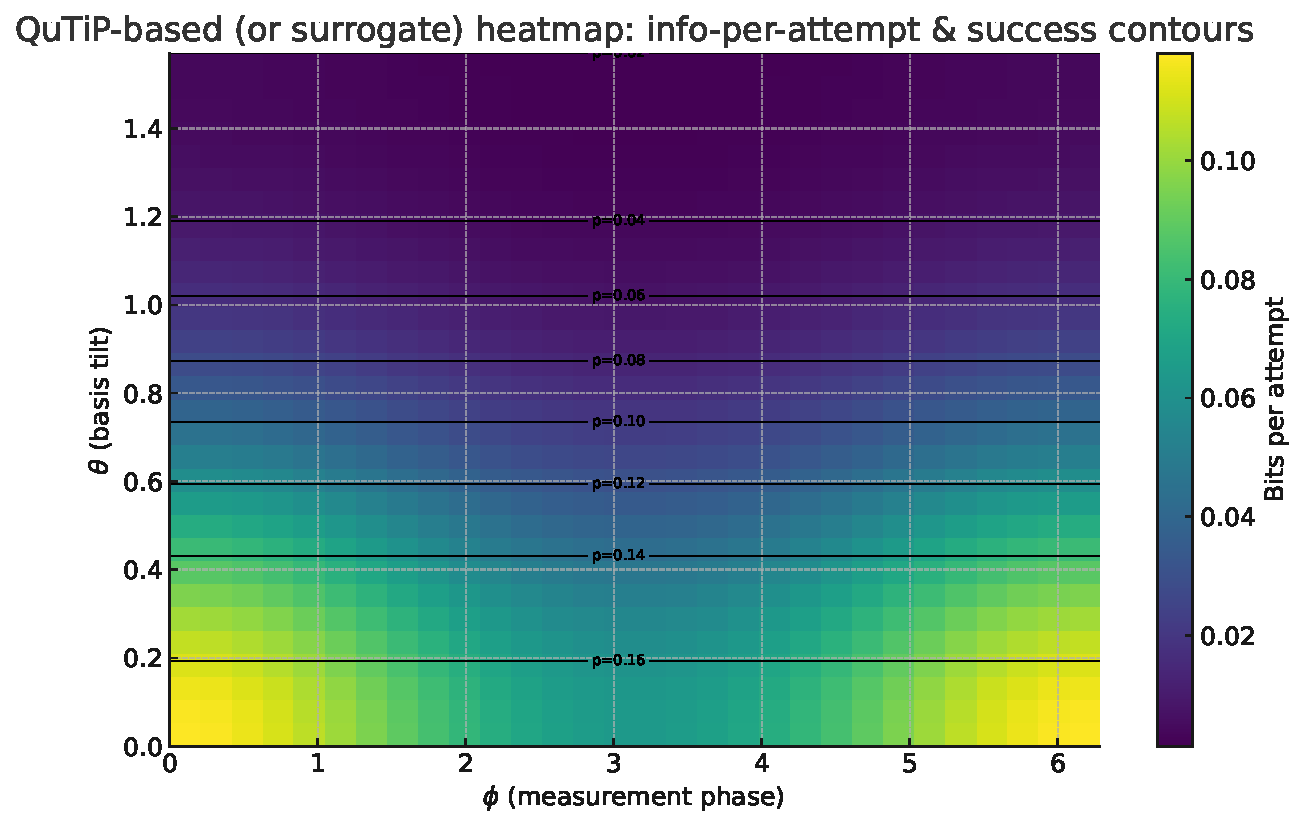
\includegraphics[width=0.75\linewidth]{figures/qutip_heatmap.pdf}
\caption{Heatmap of bits-per-attempt as a function of measurement basis $(\theta,\phi)$ with success-probability contours.}
\end{figure}


\section{Metaphysics Appendix: Histories, Identity, and Free Will}
We model the space of histories as a measurable space $(\mathcal{H},\mathcal{F})$ with prior $P_{\text{hist}}$. Consistency corresponds to an I-projection onto a feasible set $\mathcal{C}$.

\paragraph{Identity.} Let $\sigma_t$ denote a ``personal'' state evolving under morphisms $U_{t\to s}$. A retro-intervention imposes a fixed-point constraint $U_{t\to s}U_{s\to t}\sigma_t=\sigma_t$. When consistency requires redistributing probability mass over narratives, the minimum change is quantified by the Entropy Ledger.

\paragraph{Free Will (Operational).} Define $\mathsf{Free}(t):=H(A_t\mid \text{Past},\text{Ledger Info})$. Retro-resources can reduce $\mathsf{Free}$ but only by paying scarcity ($-\log\Ps$) or heat ($\mathsf{ED}$). Thus there is ``no free chronology'': influence against the arrow is always priced.


\section{Notation and Proof Outlines}
\paragraph{Loop-DPI sketch.} Normalize the non-TP retro-map $\Pi$ by conditioning on the heralded outcome. Apply a change-of-measure argument around the cycle and bound the Radon--Nikodym derivative by $1/\Ps$, yielding $\Delta I_{\circlearrowleft}\le -\log \Ps$ (bits). Finite accuracy adds a $-\log(1-\varepsilon)$ term.

\paragraph{Entropy Ledger sketch.} Consistency is enforced by projecting $P_{\text{hist}}$ onto $\mathcal{C}$ in KL. The work cost of modifying distributions obeys $\langle W\rangle\ge kT\,\KL(P\Vert P^\star)$ by Landauer and nonequilibrium work relations.


\end{document}
